\chapter{マイクロSDイメージファイル}
\label{appA}

\section{サンプル解説}
\tacsim のリポジトリのsampleディレクトリには, サンプルとして4つのマイクロSDイメージファイルが同梱されている. 

\begin{description}
    \item[TacOS-vm-8m.dmg] 仮想記憶に対応したTacOSが書き込まれた8MBのイメージファイル. カーネルと基本的なコマンドの他にsample.cmmという\cmm 言語で書かれたプログラムが入っており, {\tt c--}コマンドを実行することでコンパイルすることができる.
    \item[TacOS-vm-8m-debug.dmg] TacOS-vm-8m.dmgと同じファイルが入っているが, デバッグ用の表示をRN4020経由で出力するようになっている.
    \item[Test-8queen-8m.dmg] 8王妃問題を解くプログラムが書き込まれている8MBのイメージファイル.
    \item[Test-SioEcho-8m.dmg] シリアル通信のテストプログラムが書き込まれている8MBのイメージファイル.
\end{description}

\section{作成方法}

ここでは, MacOS上でマイクロSDイメージファイルを作成する方法を紹介する. 

\subsection{dmgファイルの作成}

Launchpadから「ディスクユーティリティ」を実行する. メニューバーから「ファイル」\rightarrow「空のイメージを作成」を選択すると, 図\ref{fig:appA-diskutil}のように, 作成するイメージファイルの設定ウィンドウが表示される.
サイズを8MB以上512MB以下, フォーマットを「MS-DOS(FAT)」, 暗号化を「なし」, パーティションを「単一パーティション - マスターブートレコード・パーティションマップ」にしてから保存. すると, dmgファイルが作成される.

\begin{figure}[H]
    \centering
    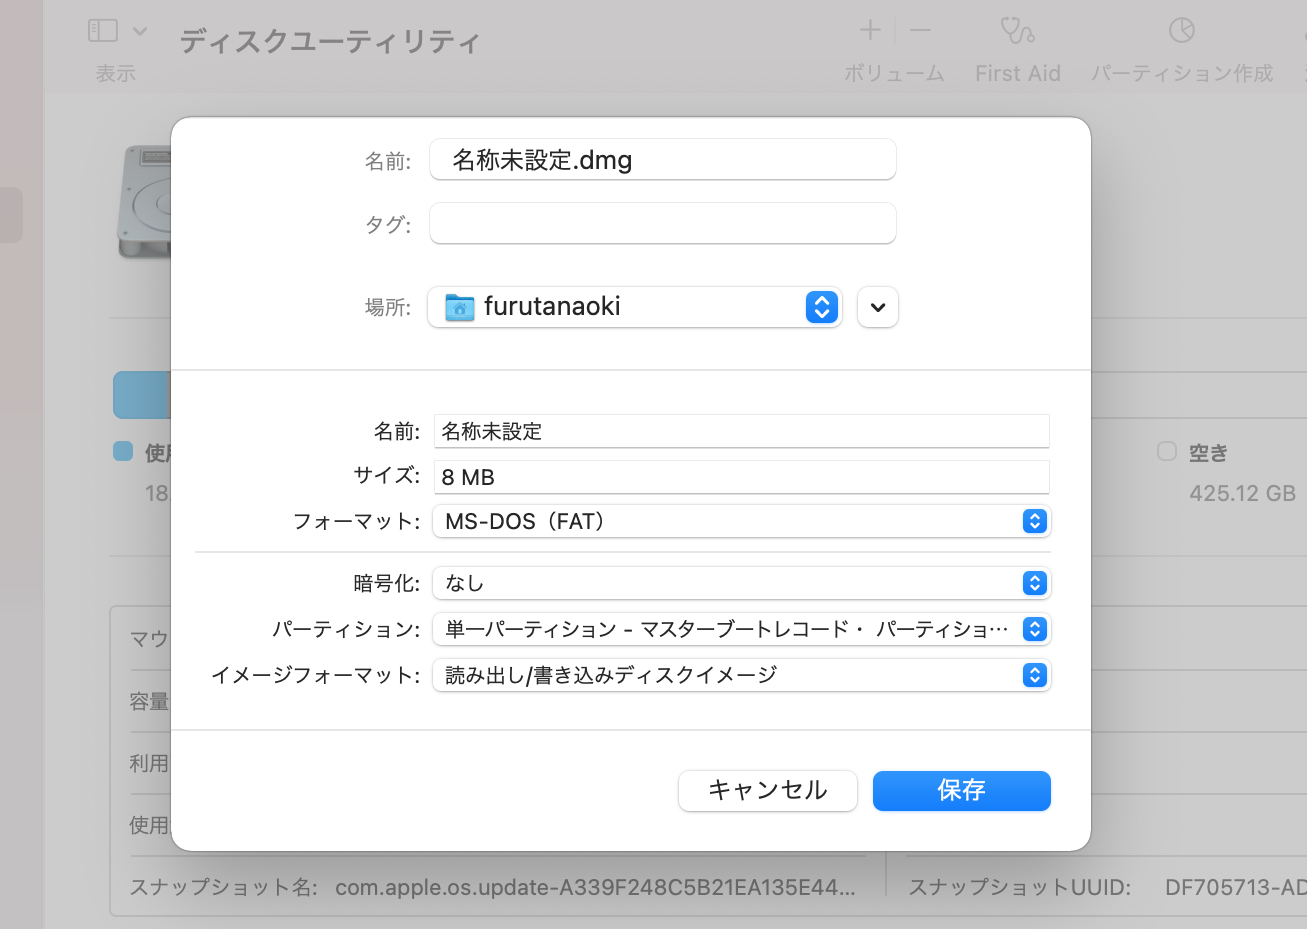
\includegraphics[width=13.5cm]{"figs/appA-diskutil.png"}
    \caption{作成するイメージファイルの設定} \label{fig:appA-diskutil}
\end{figure}

\subsection{パーティションテーブル修正}

サイズを8MB以上512MB以下にしている場合, dmgファイルのプロパティを見るとファイルシステムがFAT16であると表示されるが, パーティションテーブルのType(ファイルシステムの種類)がFAT32を表す0x0bになっているため, バイナリエディタを用いてFAT16を表す0x06に修正する必要がある. 

マニュアル通りに進めてきた場合, 520バイト目がTypeを表すバイトになっているため, そこを修正すればよい.

\begin{figure}[H]
    \centering
    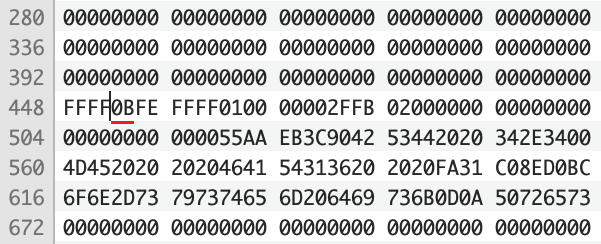
\includegraphics[width=12cm]{"figs/appA-binaryEditor.png"}
    \caption{Typeの場所} \label{fig:appA-binedit}
\end{figure}

\subsection{カーネルファイルの格納}

\tacsim で使用可能なマイクロSDイメージファイルを作成できたため, 実行したいプログラムをコンパイルし, kernel.binという名前で先程のdmgファイルの中に移動する. MacOSではdmgファイルをクリックすると自動的にマウントしてデスクトップに表示される.
